\section{Diseño de bajo nivel}
\label{low_level_design}

\subsection{Paquetes y clases concretas}
En esta sección se presentan las clases concretas que implementan las interfaces presentadas en la 
sección~\ref{high_level_design}. Para mayor claridad, se dividieron los diagramas UML por paquetes.

\subsubsection{Validator}
\par En la figura ~\ref{validator} se exhibe el diagrama de clases correspondiente al componente \textsf{validator}. Este paquete representa el módulo ``Validator'' que se observa en la figura \ref{arquitecture} en la sección ~\ref{arquitectura}.

\par La responsabilidad de este componente es realizar un control de calidad sobre las secuencias de small-RNA$_s$ determinando si las mismas se encuentran en un marco de lectura válido. Para garantizar esta calidad, es necesario traducir la cadena de nucleótidos a una cadena de aminoácidos y verificar que no queden nucleótidos libres, conocidos como \emph{codones stops}. Para ello se utilizará la librería \emph{BioPP}.

\begin{figure}[!hbtp]
	\begin{center}
		\includegraphics[width=8cm,height=5.5cm]{validator.png}
		\caption{UML - Validator}
		\label{validator}
	\end{center}
\end{figure}

\subsubsection{StatisticalControl}
\par En la figura ~\ref{statisticalControl} se observa el diagrama de clases correspondiente al componente \textsf{statisticalControl}. El mismo representa el módulo ``StatisticalControl'' que se exhibe en la figura \ref{arquitecture} en la sección ~\ref{arquitectura}.

\par La responsabilidad de este componente radica en realizar controles estadísticos sobre las secuencias de RNA$_m$. Para estos controles, será necesario la generación de secuencias random.	

\begin{figure}[!hbtp]
	\begin{center}
		\includegraphics[width=7cm,height=5.5cm]{statisticalControl.png}
		\caption{UML - StatisticalControl}
		\label{statisticalControl}
	\end{center}
\end{figure}

\subsubsection{RNAmData}
\par En la figura ~\ref{RNAmData} se observa el diagrama de clases correspondiente al componente \textsf{RNAmData}. El mismo representa el módulo ``RNAmData'' que se exhibe en la figura \ref{arquitecture} de la sección ~\ref{arquitectura}.

\par Este componente corresponde a una interface que brinda al sistema las diversas secuencias de RNA mensajero. Permite utilizar diversas fuentes de datos, en primera instancia se abarcan dos fuentes; por un lado, \emph{fasta parser} que corresponde a un archivo en formato FASTA, y por el otro (a futuro), \emph{BlastProxy} que corresponde a la obtención de secuencias a través de BLAST.	

\begin{figure}[!hbtp]
	\begin{center}
		\includegraphics[width=6.5cm,height=5.5cm]{RNAmData.png}
		\caption{UML - RNAmData}
		\label{RNAmData}
	\end{center}
\end{figure}

\subsubsection{Matcher}
\par En la figura~\ref{matching} se observa el diagrama de clases para el paquete \textsf{Matcher}. Este paquete representa el componente \textsf{Matcher} correspondiente a la figura~\ref{arquitecture} de la sección~\ref{arquitectura}.
\par La responsabilidad de este componente es realizar el matching entre secuencias y calcular el score de matching. Para ello, se generarán diversas cadenas por cada posición del RNA$_m$ resultantes de matching diferentes. 

\begin{figure}[!hbtp]
	\begin{center}
		\includegraphics[width=7cm,height=5cm]{matching.png}
		\caption{UML - Matching}
		\label{matching}
	\end{center}
\end{figure}


\subsubsection{Generator}
\par En la figura~\ref{generadorPackage} se observa el diagrama de clases para el paquete \textsf{generator} el cual corresponde al componente \textsf{generator} de figura~\ref{arquitecture} (Sección~\ref{arquitectura}).

\par La responsabilidad de este componente es brindar al sistema el servicio de \emph{``humanización''} sobre las secuencias de RNA$_m$. Para cumplir con esta responsabilidad, se ofrece al sistema el acceso al software \textsf{geneDesign} de manera independiente. 

\begin{figure}[!hbtp]
	\begin{center}
		\includegraphics[width=7cm,height=6cm]{generator.png}
		\caption{UML - Generator}
		\label{generadorPackage}
	\end{center}
\end{figure}

\subsubsection{fideo}
\par En la figura~\ref{fideopackage} se observa el diagrama de clases para el paquete \textsf{fideo}. Este paquete representa el componente \textsf{fideo} correspondiente a la figura~\ref{arquitecture} de la sección~\ref{arquitectura}.
\par La responsabilidad de este componente es brindar al sistema el servicio de \emph{``folding''} sobre secuencias de RNA$_m$. Para cumplir con esta responsabilidad, se ofrece al sistema el acceso a librerías externas de manera transparente y
permitiendo utilizar diferentes librerías para acceder a diferentes servicios. 
\par Se contemplan los siguientes tipos de folding:
\begin{itemize}
	\item RNAFold.
	\item UNAFold.
	\item MFold.
\end{itemize}
\par La importancia de este paquete y las interfaces que contiene radica en que permite abstraerse del uso de una u otra librería.

\begin{figure}[!hbtp]
	\begin{center}
		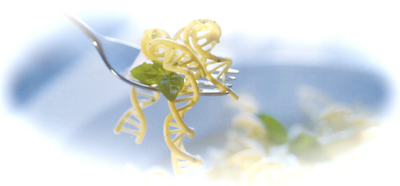
\includegraphics[width=8cm,height=6cm]{fideo.png}
		\caption{UML - fideo}
		\label{fideopackage}
	\end{center}
\end{figure}
